\chapter{格子ボルツマン法を組み込んだ深層学習モデル\label{chap:how-to-assemble}}
この章では,提案モデルの概要とより具体的な原理について説明する.

\section{提案モデルの概要}
提案モデルの概要図を図\ref{fig:overview}に示す.この図が示すように,提案モデルはLBMをベースとしている.その並進と衝突の計算に重みを導入し,予測速度と圧力に対する実際の速度と圧力との誤差からその重みを逆誤差伝播法によって学習することで,座標に依存する流体の振る舞いを精度良くシミュレーションすることを試みる.学習の流れを詳述する.まずある時刻$t_0$の各格子点上での流体の速度,圧力から,仮想粒子の分布$f(\bm{x}, \bm{v}, t_0)$を導出する.そこから数ステップに亘り,並進と衝突の計算によって仮想粒子の分布$f'(\bm{x}, \bm{v}, t+i), f(\bm{x}, \bm{v}, t+i+1) \hspace{10pt}(i=0,1,2,...)$を逐次的に得る.最終的な分布$f(\bm{x}, \bm{v}, t_1) \hspace{5pt}(t_1>t_0)$から巨視的な流体の速度と圧力を算出し,これと実際の流体の速度と圧力との誤差から,各ステップに導入した重みを逆誤差伝播法によって学習する.
\begin{figure}[htbp]
  \centering
  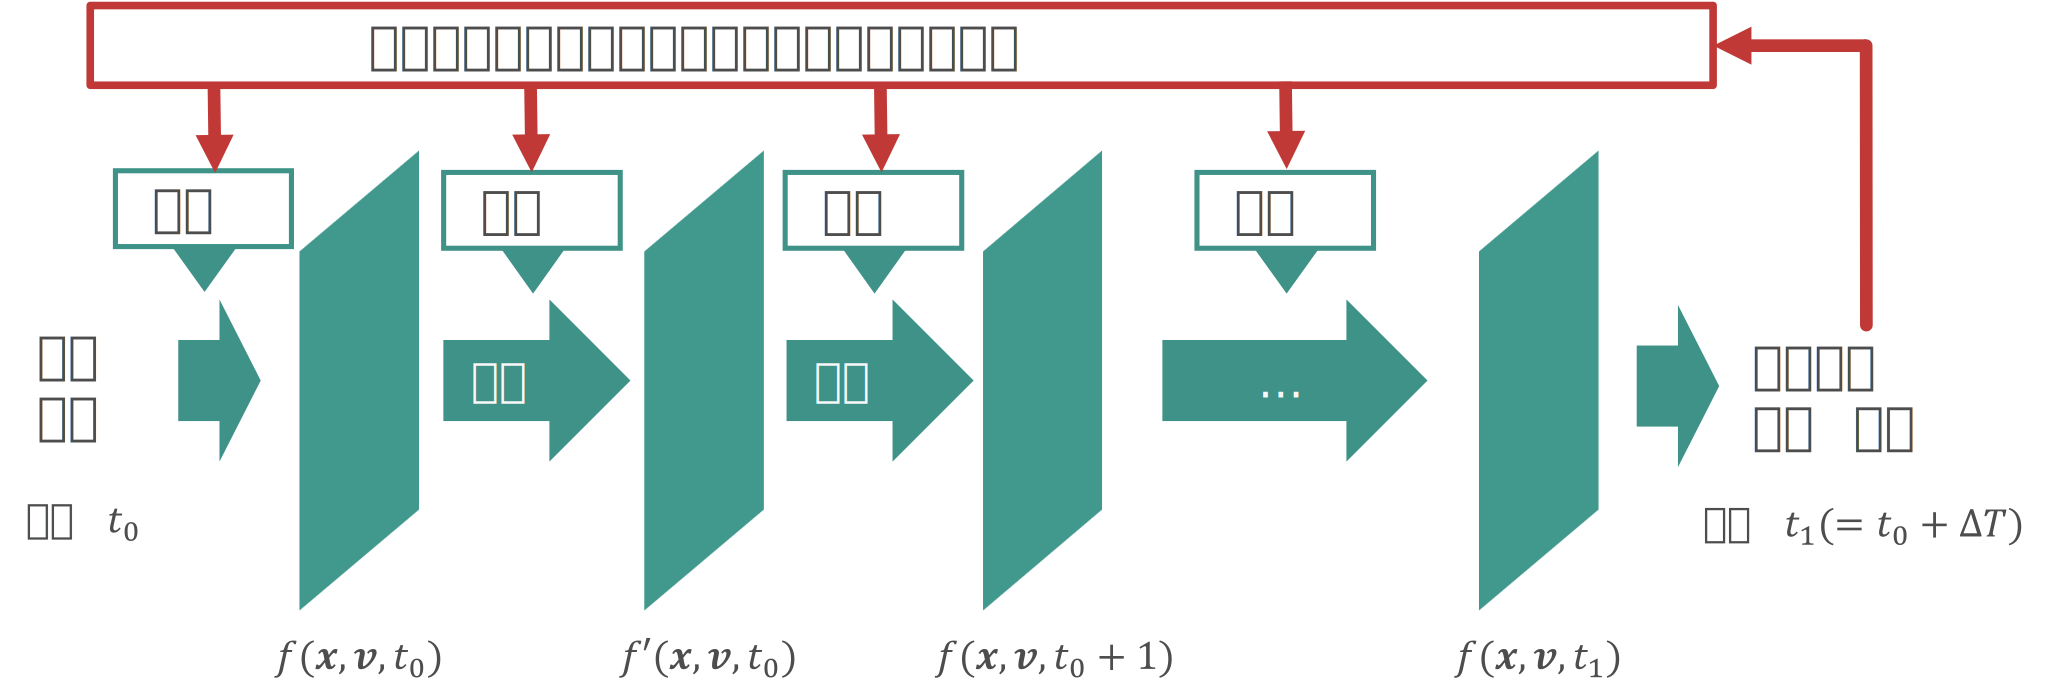
\includegraphics[width=13cm]{./how_to_assemble/figs/model_overview.svg.eps}
  \caption{提案モデルの概要図}
  \label{fig:overview}
\end{figure}

\section{提案モデルの原理}
この節では,具体的にどのようにLBMに重みを導入し学習を行うか,その原理について説明する.まずは図\ref{fig:model}(a)で表されるように,ある一時刻のデータのみが入力されたときにその3時間後の風速のみを予想する時系列性のないモデルを説明する.その後,図\ref{fig:model}(b)で表されるように3時間おきの時系列データが入力されたとき,それぞれの時刻に対して3時間後の時系列風速データを予想するモデルを説明する.

\subsection{時系列性のないモデル}
LBMの並進は,仮想粒子の分布関数$f(\bm{x}, \bm{v}, t)$を用いて以下のように表された(再掲).
\begin{equation}
  f'(\bm{x}+\bm{v}, \bm{v}, t)
  = f(\bm{x}, \bm{v}, t)
  \tag{\ref{eq:principles-streaming}}
\end{equation}

この式に重み$w'_{\rm{const}}(\bm{x}, \bm{v}, t)$, $w'_{\rm{fprev}}(\bm{x}, \bm{v}, t)$を導入する.重みを導入することで,仮想粒子の分布関数$f(\bm{x}, \bm{v}, t)$を並進させる際に,仮想粒子の流入や流出を表現することができる.重みを導入した並進の式は以下のように表される.
\begin{equation}
  f'(\bm{x}+\bm{v}, \bm{v}, t) = 
  w'_{\rm{const}}(\bm{x}, \bm{v}, t) + 
  w'_{\rm{fprev}}(\bm{x}, \bm{v}, t) f(\bm{x}, \bm{v}, t) 
  \label{eq:weighted-streaming}
\end{equation}

また,衝突の式は以下のように表された(再掲).
\begin{equation}
  f(\bm{x}, \bm{v}, t+1) = 
  f'(\bm{x}, \bm{v}, t) - 
  \frac{1}{\tau} \left[ 
    f'(\bm{x}, \bm{v}, t) - f^{eq}(\bm{x}, \bm{v}, t) 
  \right]
  \tag{\ref{eq:principles-collision}}
\end{equation}

\begin{equation}
  f^{eq}(\bm{x}, \bm{v}, t) = 
  c_i(\bm{v}) \rho(\bm{x}, t) \left[ 
    1 
    + 3\bm{v} \cdot \bm{u}(\bm{x}, t) 
    + \frac{9}{2}(\bm{v} \cdot \bm{u}(\bm{x}, t))^2 
    - \frac{3}{2}\bm{u}(\bm{x}, t)^2 
  \right]
  \tag{\ref{eq:principles-equilibrium}}
\end{equation}

これらの式にも重み$w_{\rm{fprev}}(\bm{x}, \bm{v}, t)$, $w_{\rm{vu}}(\bm{x}, \bm{v}, t)$, $w_{\rm{vxu}}(\bm{x}, \bm{v}, t)$, $w_{\rm{vu2}}(\bm{x}, \bm{v}, t)$, $w_{\rm{u2}}(\bm{x}, \bm{v}, t)$を導入する.重みを導入した衝突の式はそれぞれ以下のように表される.
\begin{equation}
  f(\bm{x}, \bm{v}, t+1) = 
  w_{\rm{fprev}}(\bm{x}, \bm{v}, t) f'(\bm{x}, \bm{v}, t) 
  + \left(1 - w_{\rm{fprev}}(\bm{x}, \bm{v}, t)\right) f^{eq}(\bm{x}, \bm{v}, t)
  \label{eq:principles-weighted-collision}
\end{equation}

\begin{equation}
\begin{split}
  f^{eq}(\bm{x}, \bm{v}, t) =
  &c_i(\bm{v}) \rho(\bm{x}, t) \\
  &[ 1 + w_{\rm{vu}}(\bm{x}, \bm{v}, t)\bm{v} \cdot \bm{u}(\bm{x}, t) \\
  &+ w_{\rm{vxu}}(\bm{x}, \bm{v}, t)\bm{v} \times \bm{u}(\bm{x}, t) \\
  &+ w_{\rm{vu2}}(\bm{x}, \bm{v}, t)(\bm{v} \cdot \bm{u}(\bm{x}, t))^2 \\
  &+ w_{\rm{u2}}(\bm{x}, \bm{v}, t)\bm{u}(\bm{x}, t)^2 ]
\end{split}
  \label{eq:principles-weighted-equilibrium}
\end{equation}

ただし,$\times$はベクトル$\bm{u} = (u_1, u_2)$, $\bm{v} = (v_1, v_2)$に対して
\begin{equation}
  \bm{u} \times \bm{v} = u_1 v_2 - u_2 v_1
  \label{eq:cross-product}
\end{equation}
と定義される演算子である.ここで,式(\ref{eq:principles-equilibrium})と比べて式(\ref{eq:principles-weighted-equilibrium})には新たに$w_{\rm{vxu}}(\bm{x}, \bm{v}, t)\bm{v} \times \bm{u}(\bm{x}, t)$という項が導入されている.これは,座標$\bm{x}$における流体の回転を表現するためである.

重みの初期値の設定として,通常のLBMと同じ係数となるように以下のように定めた.
\begin{equation}
  \left\{ \,
      \begin{aligned}
      & w'_{\rm{const}}(\bm{x}, \bm{v}, t) = 0 \\
      & w'_{\rm{fprev}}(\bm{x}, \bm{v}, t) = 1 \\
      & w_{\rm{fprev}}(\bm{x}, \bm{v}, t) = 1 - 1/\tau \\
      & w_{\rm{vu}}(\bm{x}, \bm{v}, t) = 3 \\
      & w_{\rm{vxu}}(\bm{x}, \bm{v}, t) = 0 \\
      & w_{\rm{vu2}}(\bm{x}, \bm{v}, t) = 9/2 \\
      & w_{\rm{u2}}(\bm{x}, \bm{v}, t) = -3/2
      \end{aligned}
  \right.
\end{equation}

この初期値から学習を進めることで重みを更新していく.例として,重み$w_{\rm{fprev}}(\bm{x}, \bm{v}, t)$の更新式を導出する.
